\chapter{Mechanische Modellbildung}
\label{cha:Modellbildung}
Gegenstand der Modellbildung ist die Definition von Bewegungsgleichungen zur Simulation der Roboterdynamik \cite[S.~247]{Grimble.2009}. Damit soll die aufgenommene Energie des Roboters entlang einer Bewegungsbahn bestimmt werden, ohne dass das reale System angesteuert werden muss. Zunächst erfolgt eine Beschreibung der Vorwärtskinematik mithilfe der Denavit-Hartenberg (DH) Konvention. Aufbauend darauf wird die Dynamik des Systems mithilfe des Rekursiven-Newton-Euler-Algorithmus (RNEA) formuliert.  Abschließend werden Annahmen und Vernachlässigen im Kontext der Modellbildung betrachtet.

\section{Vorwärtskinematik}
Über die Vorwärtskinematik erfolgt eine geometrische Beschreibung der Endeffektor Bewegung des Roboters entlang der kinematischen Kette\footnote{siehe Anhang \ref{add:kinematische-kette}}. Entsprechend der Gelenkvariablen wird dabei die Position und Orientierung (Pose) des Endeffektors im Basis-Koordinatensystem berechnet. Ausgehend vom Basis-Koordinatensystem werden homogene Transformationsmatrizen $\bm{A}(i) = \bm{T}^{i-1}_i \in \text{SE(3)}$\footnote{siehe Anhang \ref{add:SE3}} zwischen zwei aufeinanderfolgenden Koordinatensystemen KS$\left\{i-1\right\}$ und KS$\left\{i\right\}$ aufgestellt. Die Transformationsmatrizen sind abhängig von der Konfiguration der Gelenkvariablen $q_i$ des Roboters. 
\begin{align}
	\bm{A}_i = \bm{A}_i(q_i) 
\end{align}
Eine Repräsentation der Endeffektor-Pose $\bm{H}$ im Basis-Koordinatensystem wird über eine Multiplikation der homogenen Transformationsmatrizen entlang der kinematischen Kette erreicht. 
\begin{align}
	\label{eqn:homogeneTransformation}
	\bm{H} = \bm{T}^0_n = \bm{A}_1(q_1) ... \bm{A}_n(q_n)
\end{align}
\begin{align}
	\bm{H} =\begin{bmatrix} \bm{R}^0_n &\quad \bm{o}^0_n\\ \mathbf{0}_{1x3} &\quad 1\end{bmatrix}
\end{align}
Der Spaltenvektor $\bm{o}^0_n$ repräsentiert die Koordinaten des Ursprungs des Endeffektor-Koordinatensystems im Basis-Koordinatensystem. Die $3 \times 3 $ Matrix $\bm{R}^0_n$ entspricht der Rotation des Endeffektor-Koordinatensystems gegenüber dem Basis-Koordinatensystem. \cite[S.~75~ff.]{Spong.2020} 
\subsection*{Denavit-Hartenberg Konvention}
Eine Methode zur Bestimmung der homogenen Transformationsmatrizen ist die nach  dem Physiker Jacques Denavit und dem Ingenieur Richard Hartenberg benannte DH Konvention. Diese besagt, dass jede homogene Transformation $\bm{A}_i$ als Produkt vier nacheinander ausgeführter elementarer Transformationen, gemäß \ref{eqn:elementarTransformation} ausgedrückt werden kann. 
\begin{align}
	\label{eqn:elementarTransformation}
	\bm{A}_i &= \text{Rot}_{z,\theta_i}\text{Trans}_{z,d_i}\text{Trans}_{x,a_i}\text{Rot}_{x,\alpha_i} \\
	&= \left[\begin{matrix}
		c_{\theta_i} &\quad -s_{\theta_i} &\quad 0 &\quad 0 \\
		s_{\theta_i} &\quad c_{\theta_i} &\quad 0 &\quad 0 \\
		0 &\quad 0 &\quad 1 &\quad 0 &\quad \\ 
		0 &\quad 0 &\quad 0 &\quad 1 &\quad 
	\end{matrix}\right] 
	\left[\begin{matrix}
		1 &\quad 0 &\quad 0 &\quad 0 \\
		0 &\quad 1 &\quad 0 &\quad 0 \\
		0 &\quad 0 &\quad 1 &\quad d_i &\quad \\ 
		0 &\quad 0 &\quad 0 &\quad 1 &\quad 
	\end{matrix}\right] \notag \\
	& \times
	\left[\begin{matrix}
		1 &\quad 0 &\quad 0 &\quad a_i \\
		0 &\quad c_{\alpha_i} &\quad -s_{\alpha_i} &\quad 0 \\
		0 &\quad s_{\alpha_i} &\quad c_{\alpha_i} &\quad 0 &\quad \\ 
		0 &\quad 0 &\quad 0 &\quad 1 &\quad 
	\end{matrix}\right]
	\left[\begin{matrix}
		1 &\quad 0 &\quad 0 &\quad 0 \\
		0 &\quad 1 &\quad 0 &\quad 0 \\
		0 &\quad 0 &\quad 1 &\quad 0 &\quad \\ 
		0 &\quad 0 &\quad 0 &\quad 1 &\quad 
	\end{matrix}\right]
	\notag \\
	c = cos\notag \\
	s = sin \notag 
\end{align}
Die Parameter entsprechen dem Gelenkwinkel $\theta_i$, dem Gelenkabstand $d_i$, der Armelementlänge $a_i$ und der Verwindung $\alpha_i$, wobei $d_i$, $a_i$ und $\alpha_i$ konstant sind. \cite[S.~79]{Spong.2020}
%
\subsection*{Festlegung der Koordinatensysteme}
Abbildung \ref{fig:kr210} zeigt den zu untersuchenden KUKA KR210 R2700-2 Industrieroboter. Die Bezeichnung der Maschine gibt Auskunft über ihre technischen Daten.  Die Nenn-Traglast beträgt 210 kg. Die maximale Reichweite des Roboters liegt bei 2701 mm. Weitere Informationen sind dem Datenblatt, siehe Anhang \ref{add:datenblatt}, zu entnehmen.  

\begin{figure}[tbph]
	\centering
	\includegraphics[width=0.8\linewidth]{images/KR210}
	\caption{KUKA KR210 R2700-2}
	\label{fig:kr210}
\end{figure}

Im ersten Schritt werden die Achsen $z_i, \ i = 0,...,n-1, n=6$, siehe Abbildung \ref{fig:zachsen}, definiert. Im zweiten Schritt wird das Basiskoordinatensystem ${0}$ festgelegt, wobei der Ursprung $\bm{o}_0$ auf der Achse $z_0$ platziert wird. Die Definition des ersten Koordinatensystems entspricht dem vom Hersteller festgelegten ROBROOT-Koordinatensystem. Dies erlaubt eine Überprüfung der Vorwärtskinematik mithilfe der, von der KUKA Robotersteuerung (KUKA Robot Control (KR C)) berechneten kartesischen Koordinaten. Des Weiteren werden, siehe Abbildung \ref{fig:KS}, aufsteigend die Koordinatensysteme KS$\{i\},i=1,...,n-1$ basierend auf KS$\left\{i-1\right\}$, sowie das rot hervorgehobene Endeffektor-Koordinatensystem $0_6x_6y_6z_6$ platziert. Ein Werkzeug ist am Versuchsroboter nicht verbaut. Das Endeffektor-KS liegt auf dem Flansch.

Es werden dabei folgende Regeln berücksichtigt.  

\begin{figure}[tbph]
	\centering
	\includegraphics[width=0.5\linewidth]{images/zAchsen}
	\caption[]{Festlegung der z-Achsen}
	\label{fig:zachsen}
\end{figure}
%
\begin{figure}[tbph]
	\centering
	\includegraphics[width=0.5\linewidth]{images/KS}
	\caption{DH-Konvention - Festlegung der Koordinatensysteme}
	\label{fig:KS}
\end{figure}

\begin{itemize}
	\item Falls sich $z_i$ und $z_{i-1}$ schneiden, ist der Ursprung $\bm{o}_i$ in den Schnittpunkt zu legen. Die Achse $x_i$ wird rechtwinklig zur $z_{i-1}-z_i$-Ebene definiert.\footnote{gilt für KS$\left\{4\right\}$ und KS$\left\{5\right\}$} 
	\item Falls  $z_i$ und $z_{i-1}$ parallel sind, wird der Ursprung $\bm{o}_i$ auf die Achse $z_i$ gelegt. Die Achse $x_i$ wird parallel zur gemeinsamen Normale von $z_i$ und $z_{i-1}$	im Punkt $\bm{o}_i$ definiert.\footnote{gilt für KS$\left\{2\right\}$} 
	\item Falls  $z_i$ und $z_{i-1}$ nicht koplanar sind, wird der Ursprung $\bm{o}_i$ auf den Schnittpunkt der Achse $z_i$ mit der gemeinsamen Normalen von $z_i$ und $z_{i-1}$  gelegt. Die Achse $x_i$ ist die gemeinsamen Normale von $z_i$ und $z_{i-1}$.\footnote{gilt für KS$\left\{1\right\}$ und KS$\left\{3\right\}$}
	\item die Achse $y_i$ vervollständigt das rechtshändige, kartesische Koordinatensystem
\end{itemize} 
%
Im nächsten Schritt erfolgt die Identifizierung der DH-Parameter.  $\theta_i$ entspricht der Rotation um $z_{i-1}$, sodass $x_{i-1}||x_i$. Der Parameter $d_i$ drückt die Translation entlang $z_{i_1}$ bis zum Schnittpunkt S von $z_{i-1}$ und $x_i$ aus. Der Parameter $a_i$ entspricht der Translation entlang $x_i$, um den Schnittpunkt S in den Ursprung $o_i$ zu überführen. Abschließend ist $\alpha_i$ die Rotation um $x_i$, zur Überführung von $z_{i-1}$ in $z_i$. Aus den Elementartransformationen, siehe Gleichung \ref{eqn:elementarTransformation}, wird die Gesamttransformationen entsprechend \ref{eqn:homogeneTransformation} berechnet. Tabelle \ref{tab:dh} listet die identifizierten DH-Parameter. 

\begin{table}[tbph]
	\centering
	\caption{Denavit-Hartenberg Parameter}
	\label{tab:dh}
	\begin{tabular}{|c|c|c|c|c|}
		\hline
		Gelenk & $\theta$ [$^\circ$] & $d$ [m] & $a$ [m] & $\alpha$ [$^\circ$]\\
		\hline
		1& 0 & 0,645 & 0,330 & $-90$ \\
		\hline
		2& $-90$ & 0 & 1,150 & 0 \\
		\hline
		3& 0 & 0 & 0,115 & $90$ \\
		\hline
		4& 0 & -1,220 & 0 & $-90$ \\
		\hline
		5& 0 & 0 & 0 & $-90$ \\
		\hline
		6& $90$ & 0,215 & 0 & 0 \\
		\hline
	\end{tabular}
\end{table}

%Eine Verarbeitung der Gelenkwinkel, welche in der KR C für eine bestimmte Pose definiert sind, bedingt eine Anpassung DH-Parameter. 
Der Roboterhersteller definiert die Drehrichtung der Achse $z_{1}$ invertiert gegenüber. der o. g. Festlegung. Folglich werden die vor der Robotersteuerung bereitgestellten Winkel des ersten Gelenks  mit -1 multipliziert, bevor eine Weiterverarbeitung im Modell erfolgt. Des Weiteren werden vom dritten Gelenkwinkel 90° subtrahiert, bevor der Wert dem Modell übergeben wird. Die Vorwärtskinematik wurde über drei Posen am realen System verifiziert. Dabei ist festzustellen, dass die Robotersteuerung eine Elastizität der Verbindungsglieder berücksichtigt, wohingegen in der Modellbeschreibung von starren Körpern ausgegangen wird. Die Implementierung der DH-Transformation ist im Anhang \ref{add:dh}  aufgeführt. 
%
\section{Geschwindigkeits-Kinematik}
Die Geschwindigkeits-Kinematik definiert die lineare Endeffektor-Geschwindigkeit und die  Endeffektor-Winkelgeschwindigkeit in Abh{\"a}ngigkeit der Gelenkwinkelgeschwindigkeiten des Roboters. Eine mathematische Beschreibung des Zusammenhangs erfolgt {\"u}ber die Jacobi-Matrix der Vorw{\"a}rtskinematik \cite[S.~101]{Spong.2020}. Grundlegende Definitionen zur Aufstellung der Jacobi-Matrizen $\bm{J}_v$ und $\bm{J}_{\omega}$ werden im Anhang  \ref{add:geschwindigkeitskinematik} betrachtet. 
%
\section{Dynamik}
Ziel des Kapitels ist die Berechnung der aufzubringenden Momente in den sechs Gelenken des Roboters bei Ansteuerung entlang einer Bewegungsbahn.
Der dynamische Zusammenhang zwischen Gelenkkräften und Gelenkbewegungen wird zunächst formal mithilfe der Euler-Lagrange Gleichungen formuliert. Anschließend folgt die numerisch effiziente Implementierung  über den RNEA \cite[S.~247]{Grimble.2009}. 
%
\subsection{Euler-Lagrange Gleichungen}
Die Lagrange Funktion $L$ eines mechanischen Systems entspricht der Differenz der kinetischen Energie $K$ und der potentiellen Energie $U$ \cite[S.~175]{Spong.2020}. 
\begin{equation}
	L = K-U 
\end{equation}
%
%Für einen bewegten Starrkörper mit der Geschwindigkeit $\dot{q}$ und Masse $m$ folgt unter Einwirkung der Fallbeschleunigung $g$ die Formulierung. 
%
%\begin{equation}
%	L = \dfrac{1}{2}m\dot{q}^2 - mgq
%\end{equation}
%
Die Euler-Lagrange-Gleichung wird über den folgenden Ausdruck beschrieben. Dabei entspricht die Ordnung $n$ des Systems der Anzahl generalisierter Koordinaten\footnote{Voneinander unabhängige Koordinaten, welche den aktuellen Systemzustand vollständig beschreiben \cite{Engelke.2008}}, bzw. im Anwendungsfall den sechs rotatorischen Gelenkkoordinaten ($\theta_1$,...,$\theta_6$). Die Größe $\bm{\tau}$ repräsentiert generalisierte Kräfte\footnote{Kräfte und Momente}. Im Anwendungsfall werden die Antriebsmomente in den Gelenken betrachtet. 
%
\begin{equation}
	\dfrac{d}{dt} \dfrac{\partial{L}}{\partial{\dot{{q}_i}}}- \dfrac{\partial{L}}{\partial{{q}_i}} = {\tau}_i \ ;  \ i = 1,...,n 
\end{equation}
%
\begin{equation}
	\dfrac{\partial{L}}{\partial{\dot{\bm{q}}}} = \dfrac{\partial{K}}{\partial{\dot{\bm{q}}}}
\end{equation}
%
\begin{equation}
	\dfrac{\partial{L}}{\partial{\bm{q}}} = -\dfrac{\partial{U}}{\partial{\bm{q}}}
\end{equation}
%
Die kinetischen Energie des Roboters entspricht der Gleichung  \ref{eqn:ekin}
\begin{equation}
	\label{eqn:ekin}
	K = \dfrac{1}{2} \dot{\bm{\bm{q}}}^T \left[\sum_{i=1}^{n} \left( m_i \bm{J}_{v_i}(\bm{q})^T \bm{J}_{v_i}(\bm{q}) + \bm{J}_{\omega_i}(\bm{q})^T \bm{R}^0_i(\bm{q}) \bm{I}^{i}_{i} \bm{R}^0_i(\bm{q})^T \bm{J}_{\omega_i}(\bm{q}) \right) \right]\dot{\bm{\bm{q}}}
\end{equation}
%
Der Ausdruck in der Klammer wird als Massenmatrix $\bm{M}(\bm{q})$ bezeichnet. 
Die Massen $m_i$ wurden über ein Computer Aided Design- (CAD) Modell, welches vom Hersteller bereitgestellt wird, identifiziert. 
Die Trägheitstensoren $\bm{I}^{i}_{i}$, bezogen auf den Masseschwerpunkt des Verbindungsglieds $i$, sind relativ zu den Gelenkkoordinatensystemen orientiert und damit für alle Konfigurationen des Roboters konstant. 
Über das CAD-Modell werden die Trägheitstensoren $\bm{I}^{0}_{i}$ relativ zum KS$\left\{0\right\}$ bereitgestellt. Die gewünschte Umrechnung erfolgt mithilfe der Ähnlichkeitstransformation \ref{eqn:similarity}.
%
\begin{equation}
	\label{eqn:similarity}
	\bm{I}^{i}_{i} = {\bm{R}^{0}_i}^T \bm{I}^{0}_{i} \bm{R}^0_i
\end{equation}
%
Die potentielle Energie wird über den Ausdruck \ref{eqn:epot} berechnet.
%
\begin{equation}
	\label{eqn:epot}
	U = \sum_{i=1}^{n} m_i \bm{g}^T\bm{r^0_{C_i}}
\end{equation}
%
Der Vektor $\bm{g} = [0~0-9,81]^T~\dfrac{\text{m}}{\text{s}}$ ist die Fallbeschleunigung, ausgedrückt in KS$\left\{0\right\}$. Der Vektor $\bm{r}^0_{C_i}$ definiert die Lage des Masseschwerpunkts vom Verbindungsglied $i$ im  KS$\left\{0\right\}$. Für die Herleitung der Bewegungsgleichungen \ref{eqn:bewegungsgleichungen} wird auf die Literatur \cite[S.~180 ff.]{Spong.2020} verwiesen. Hierbei ist ersichtlich, dass die numerische Bestimmung von $\bm{\tau}$ aufgrund der partiellen Ableitungen von $K$ und $U$ insbesondere in den letzten Gliedern der kinematischen Kette einen hohen Berechnungsaufwand erfordert, weshalb das Modell über den RNEA implementiert ist. 
%
\begin{equation}
	\label{eqn:bewegungsgleichungen}
	\bm{M}(\bm{q})\ddot{\bm{q}} + \bm{C}(\bm{q},\dot{\bm{q}})\dot{\bm{q}} + \bm{g}(\bm{q}) = \bm{\tau}
\end{equation}
%
Der Term $\bm{C}(\bm{q},\dot{\bm{q}})\dot{\bm{q}}$ berücksichtigt die Einflüsse der Corioliskraft und Zentrifugalkraft\footnote{Eine detaillierte Betrachtung von Scheinkräften in rotierenden Bezugssystemen erfolgt in  \cite[S.~159]{Roth.2016}}. Der Vektor $\bm{g}(\bm{q})$ berücksichtigt die Gravitation. \cite[S.~180~ff.]{Spong.2020}
%
\subsection{Rekursiver-Newton-Euler-Algorithmus}
%
Der Ansatz sieht vor, jedes Verbindungsglied der kinematischen Kette und die auf darauf wirkenden Kräfte $-\boldsymbol{f}_{i+1} $ und $ \boldsymbol{f}_i $ im Einzelfall zu betrachten. Ziel ist die Berechnung der im zugehörigen Gelenk wirkenden Drehmomente $\bm{\tau}$. Zur Berechnung der Drehmomente $\bm{\tau}$ in den Gelenken wird der Vektor $\bm{\mu}$ eingeführt. $\bm{\mu}_i$ hat die Dimension $3 \times n$ und repräsentiert das Drehmoment im Gelenk $i$ des Verbindungsglieds $i$. $\bm{\tau}_i$ entspricht dem Betrag des Drehmoments je Gelenk $i$. Abbildung \ref{fig:rnea} zeigt die, zu berücksichtigenden Größen am Beispiel eines generischen Verbindungsglieds $i$.

\begin{figure}[tbph]
	\centering
	\includegraphics[width=1\linewidth]{images/rnea}
	\caption{Generisches Verbindungsglied \cite[S.~283]{Grimble.2009}}
	\label{fig:rnea}
\end{figure} 

\subsubsection*{Kräfte und Momente}
\setlist{noitemsep}
\begin{itemize}
	\item $ \boldsymbol{f}_i $ - Kraft, die vom Verbindungsglied $ i-1 $ auf das Verbindungsglied $ i $ ausgeübt wird
	\item $ -\boldsymbol{f}_{i+1} $ - Kraft, die vom Verbindungsglied $ i+1 $ auf das Verbindungsglied $ i $ ausgeübt wird
	\item $ \boldsymbol{\mu}_i $ - Drehmoment, welches vom Verbindungsglied $ i-1 $ auf das Verbindungsglied $ i $ ausgeübt wird
	\item $ -\boldsymbol{\mu}_{i+1} $ - Drehmoment, welches vom Verbindungsglied $ i+1 $ auf das Verbindungsglied $ i $ ausgeübt wird
\end{itemize}
%
In der MATLAB\textsuperscript{\textregistered} Implementierung des RNEA werden alle Größen  des Verbindungsglieds $i$ auf das  fest damit verbundenen KS$\left\{i\right\}$ bezogen. Daraus resultieren die Kräfte und Momente in der Notation $\boldsymbol{f}_{i}^{i} $ und $ \boldsymbol{\mu}_i^{i} $. Nachfolgend werden die Parameter der Verbindungsglieder eingeführt. Die Werte der Systemparameter sind im Anhang \ref{add:Systemparameterdef} aufgeführt.
%
\subsubsection*{Parameter}
\setlist{noitemsep}
\begin{itemize}
	\item $ m_i $ - Masse des Verbindungsglieds $i$
	\item $ \bm{I}^{i}_{i} $ - Trägheitstensor des Verbindungsglieds $i$ im fest damit verbundenen KS$\left\{i\right\}$ 
	\item $ \boldsymbol{r}^{i}_{i-1,C_i} $ - Vektor vom Ursprung des KS$\left\{i-1\right\}$ zum Masseschwerpunkt $ C_i $ des Verbindungsglieds $i$ ausgedrückt in KS$\left\{i\right\}$ 
	\item $ \boldsymbol{r}^{i}_{i,C_i} $ - Vektor vom Ursprung des KS$\left\{i\right\}$ zum Masseschwerpunkt $ C_i $ ausgedrückt in KS$\left\{i\right\}$ 
	\item $ \boldsymbol{r}^{i}_{i-1,i} $ - Vektor vom Ursprung des KS$\left\{i-1\right\}$ zum Ursprung des  KS$\left\{i\right\}$ ausgedrückt in KS$\left\{i\right\}$ 
	\item $ i_i$ - Übersetzungsverhältnis des Getriebes $i$
\end{itemize}
%
\subsubsection*{Geschwindigkeiten und Beschleunigungen}
\setlist{noitemsep}
\begin{itemize}
	\item $ \dot{\boldsymbol{p}}_{C_i} $ - Lineare Geschwindigkeit im Masseschwerpunkt $ C_i $ 
	\item $ \dot{\boldsymbol{p}}_i $ - Lineare Geschwindigkeit im Ursprung des KS$\left\{i\right\}$
	\item $ \boldsymbol{\omega}_i $ - Winkelgeschwindigkeit des Verbindungsglieds $i$
	\item $ \ddot{\boldsymbol{p}}_{C_i} $ - Lineare Beschleunigung im Masseschwerpunkt $ C_i $
	\item $ \ddot{\boldsymbol{p}}_i $ - Lineare Beschleunigung im Ursprung des KS$\left\{i\right\}$
	\item $ \boldsymbol{\dot{\omega}}_i $ - Winkelbeschleunigung des Verbindungsglieds $i$
\end{itemize}
%
Mit Kenntnis der Größen $\bm{q}, \dot{\bm{q}}, \ddot{\bm{q}}$ und unter Festlegung der Startbedingungen $\bm{\omega}_0 = 0,~ \ddot{\bm{p}_0}-g = [0~0-9.81]^T~\text{und}~ \ddot{\bm{\omega}_0} = 0$  erfolgt sukzessive die Berechnung der Geschwindigkeiten und Beschleunigungen für jedes Verbindungsglied, beginnend mit dem ersten. 
Die Gleichungen \ref{eqn:rnea0}, \ref{eqn:rnea1}, \ref{eqn:rnea2} und  \ref{eqn:rnea3} sind der Literatur  \cite[S.~287~f.]{Grimble.2009} entnommenen. Der betrachtete KUKA KR210 R2700-2 weist eine RRR-Kinematik\footnote{Drei rotatorische Gelenke} mit Zentralhand\footnote{Funktionsumfang Rollen, Nicken, Gieren} auf weshalb eine Beschreibung für rotatorische Gelenke gewählte wurde.
%
\begin{equation}
	\label{eqn:rnea0}
	\bm{\omega}^i_i = {\bm{R}^{i-1}_i}^T  \left( \bm{\omega}^{i-1}_{i-1} +\dot{\theta}_i\bm{z_0} \right)
\end{equation}
%
\begin{equation}
	\label{eqn:rnea1}
	\dot{\bm{\omega}}^i_i = {\bm{R}^{i-1}_i}^T  \left( \dot{\bm{\omega}}^{i-1}_{i-1} +\ddot{\theta}_i\bm{z_0} +\dot{{\theta}}_i\bm{\omega}^{i-1}_{i-1} \times \bm{z}_0 \right)
\end{equation}
%
\begin{equation}
	\label{eqn:rnea2}
	\ddot{\bm{p}}^i_i = {\bm{R}^{i-1}_i}^T  \ddot{\bm{p}}^{i-1}_{i-1} + \dot{\bm{\omega}}^{i}_{i} \times \bm{r}^{i}_{i-1,i} + {\bm{\omega}}^{i}_{i} \times \left(  {\bm{\omega}}^{i}_{i} \times \bm{r}^{i}_{i-1,i} \right)
\end{equation}
%
\begin{equation}
	\label{eqn:rnea3}
	\ddot{\bm{p}}^i_{C_i} = \ddot{\bm{p}}^{i}_{i} + \dot{\bm{\omega}}^{i}_{i} \times \bm{r}^{i}_{i,C_i} + {\bm{\omega}}^{i}_{i} \times \left(  {\bm{\omega}}^{i}_{i} \times \bm{r}^{i}_{i,C_i} \right)
\end{equation}
%
Im nächsten Schritt erfolgt die rekursive Berechnung der Kräfte und Drehmomente. Der Algorithmus beginnt mit der Berechnung der Größen für das sechste Gelenk, gemäß der Gleichungen \ref{eqn:rnea4}, \ref{eqn:rnea5} und \ref{eqn:rnea6}. $\bm{f}^{n+1}_{n+1}$ und $\bm{\mu}^{n+1}_{n+1}$ werden zu 0 angenommen. 
%
\begin{equation}
	\label{eqn:rnea4}
	\bm{f}^{i}_{i} = \bm{R}^{i}_{i+1} \bm{f}^{i+1}_{i+1} + m_i\ddot{\bm{p}}^{i}_{C_i}
\end{equation}
%
\begin{equation}
	\label{eqn:rnea5}
	\bm{\mu}^{i}_{i} = -\bm{f}^{i}_{i} \times \left( \bm{r}^{i}_{i-1,i} + \bm{r}^{i}_{i,C_i} \right) + \bm{R}^{i}_{i+1} \bm{\mu}^{i+1}_{i+1} + \bm{R}^{i}_{i+1} \bm{f}^{i+1}_{i+1} \times \bm{r}^{i}_{i,C_i} + \bm{I}^{i}_{i} \dot{\bm{\omega}}^{i}_{i} + {\bm{\omega}}^{i}_{i} \times (\bm{I}^{i}_{i}{\bm{\omega}}^{i}_{i})
\end{equation}
%%
\begin{equation}
	\label{eqn:rnea6}
	\tau_i = i_i{\bm{\mu}^{i}_{i}}^T {\bm{R}^{i-1}_{i}}^T [0~0~1]^T
\end{equation}
%
Aufgrund der Lagerausführung des ersten Gelenks wird angenommen, dass das nachfolgende Drehmoment nicht auf das erste Gelenk übertragen wird, sodass der Term $\bm{R}^{i}_{i+1} \bm{\mu}^{i+1}_{i+1}$ hierbei entfällt. Aus den identifizierten Drehmomenten $\tau_i$ erfolgt durch Multiplikation mit den Winkelgeschwindigkeiten $\dot{{d}}$ die Berechnung der mechanischen Leistung $P_{mech}$. Die Implementierung des Modells ist dem Anhang \ref{add:rnea} zu entnehmen. \cite[S.~282~ff.]{Grimble.2009}
%
\section{Modellannahmen und Vernachlässigungen}
Bei der Entwicklung des mechanischen Modells zur Simulation der Roboterdynamik wurden Annahmen getroffen um die Komplexität zu reduzieren. Ein wesentlicher Einfluss ist der Vernachlässigung des hydraulischen Gewichtsausgleichs am zweiten Gelenk zuzuschreiben. Der Gewichtsausgleich ist aus einem Hydraulikzylinder mit Membranspeicher aufgebaut und wirkt dem am zweiten Gelenk auftretenden Drehmoment entgegen. Im Modell wurde dieser aufgrund fehlender Konstruktionsdaten bezüglich des Kolbendurchmessers und Kolbenstangendurchmessers nicht berücksichtigt. Fehlende Daten sind auch der Grund für die Auslassung des Gewichts und der Steifigkeit der Schlauchpakete. Das Gewicht der Elektromotoren\footnote{Gemeint ist der Stator}  wird ebenfalls vernachlässigt. Aufgrund des Verhältnisses zwischen der Masse der Motoren und dem Gewicht der Achsen  wird diese Vernachlässigung toleriert. Am Beispiel des dritten Verbindungsglieds beträgt das Verhältnis 1:15.  Die gleiche Schlussfolgerung gilt für die Massenträgheit der Motoren\footnote{Gemeint ist der Rotor}. \cite[S.~287~f.]{Grimble.2009} berücksichtigt bei der Berechnung der Drehmomente zudem die Einflüsse der viskosen und der coloumbschen Reibung. Die entsprechenden Reibungskoeffizienten werden im Modell nicht berücksichtigt. Neben der Berechnung der mechanisch aufzuwendenden Leistung erfordert eine hohe Modellgenauigkeit die Betrachtung der elektrischen Komponenten in Abbildung \ref{fig:zk}. Bei den Motoren handelt es sich um dreiphasige permanentmagneterregte Synchronmaschinen (PMSM).  Die Ansteuerung erfolgt über Frequenzumrichter. Im Ersatzschaltbild (ESB) sind alle Antriebe über einen gemeinsamen Gleichrichter vom Netz auf einen Gleichspannungszwischenkreis gekoppelt. PMSM können sowohl motorisch als auch generatorisch betrieben werden. Für die Berechnung des Energieverbrauchs in der vorliegenden Arbeit wird angenommen, dass die generatorisch umgewandelte Energie über einen Bremswiderstand als Wärme abgeführt wird. Von einer Spannungs-Schwellwert gesteuerten Zu- und Abschaltung des Bremswiderstands wird abgesehen. \cite[S.~21~ff.]{Eggers.2019}

\begin{figure}[tbph]
	\centering
	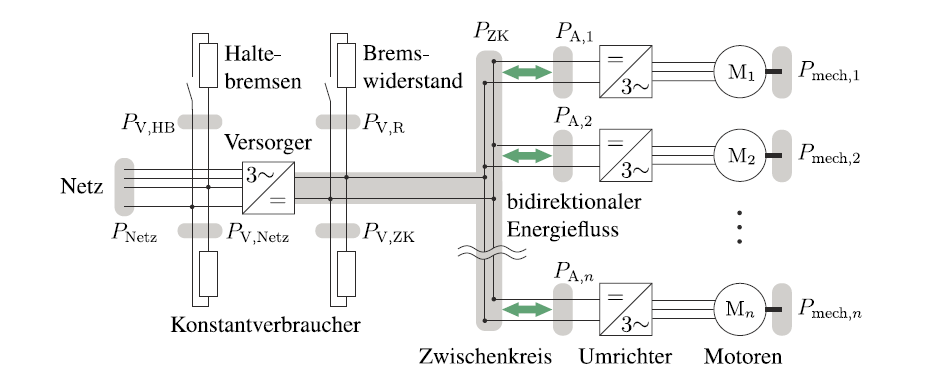
\includegraphics[width=1\linewidth]{images/zk}
	\caption{Ersatzschaltbild der aufgenommenen Netzleistung \cite[S.~20]{Eggers.2019}}
	\label{fig:zk}
\end{figure}